\section{Parameter Identification: Black Box Model}

\begin{frame}[c]
	\frametitle{Motivation}
	\begin{columns}[c]
		\column{.5\textwidth}
			\onslide<1->
			\textbf{Examples}
			\begin{itemize}
				\item{Friction coefficients}
				\item{Masses}
				\item{Inertia}
			\end{itemize}
			
			\vspace{.5cm}
			
			\onslide<2->
			\textbf{Black box model}
			\begin{itemize}
				\item{Realistic model from Siemens}
				\item{Confidential information}
			\end{itemize}
		\column{.5\textwidth}
			\centering
			\includegraphics<1-2>[width=\linewidth]{img/Blackbox_0}
			\includegraphics<3>[width=\linewidth]{img/Blackbox_1}
			\includegraphics<4>[width=\linewidth]{img/Blackbox_2}
			\includegraphics<5>[width=\linewidth]{img/Blackbox_3}
			\includegraphics<6->[width=\linewidth]{img/Blackbox_4}
	\end{columns}
\end{frame}

\begin{frame}[c]
	\frametitle{Trajectories}
	\textbf{Input:} Joystick commands for Up/Down and Forth/Back \\
	\vspace{.4cm}
	\textbf{Output:} Position of the shovel
	\vspace{-.3cm}
	\begin{columns}[T]
		\column{.5\textwidth}
		\onslide<2->
		\begin{figure}
			\centering
			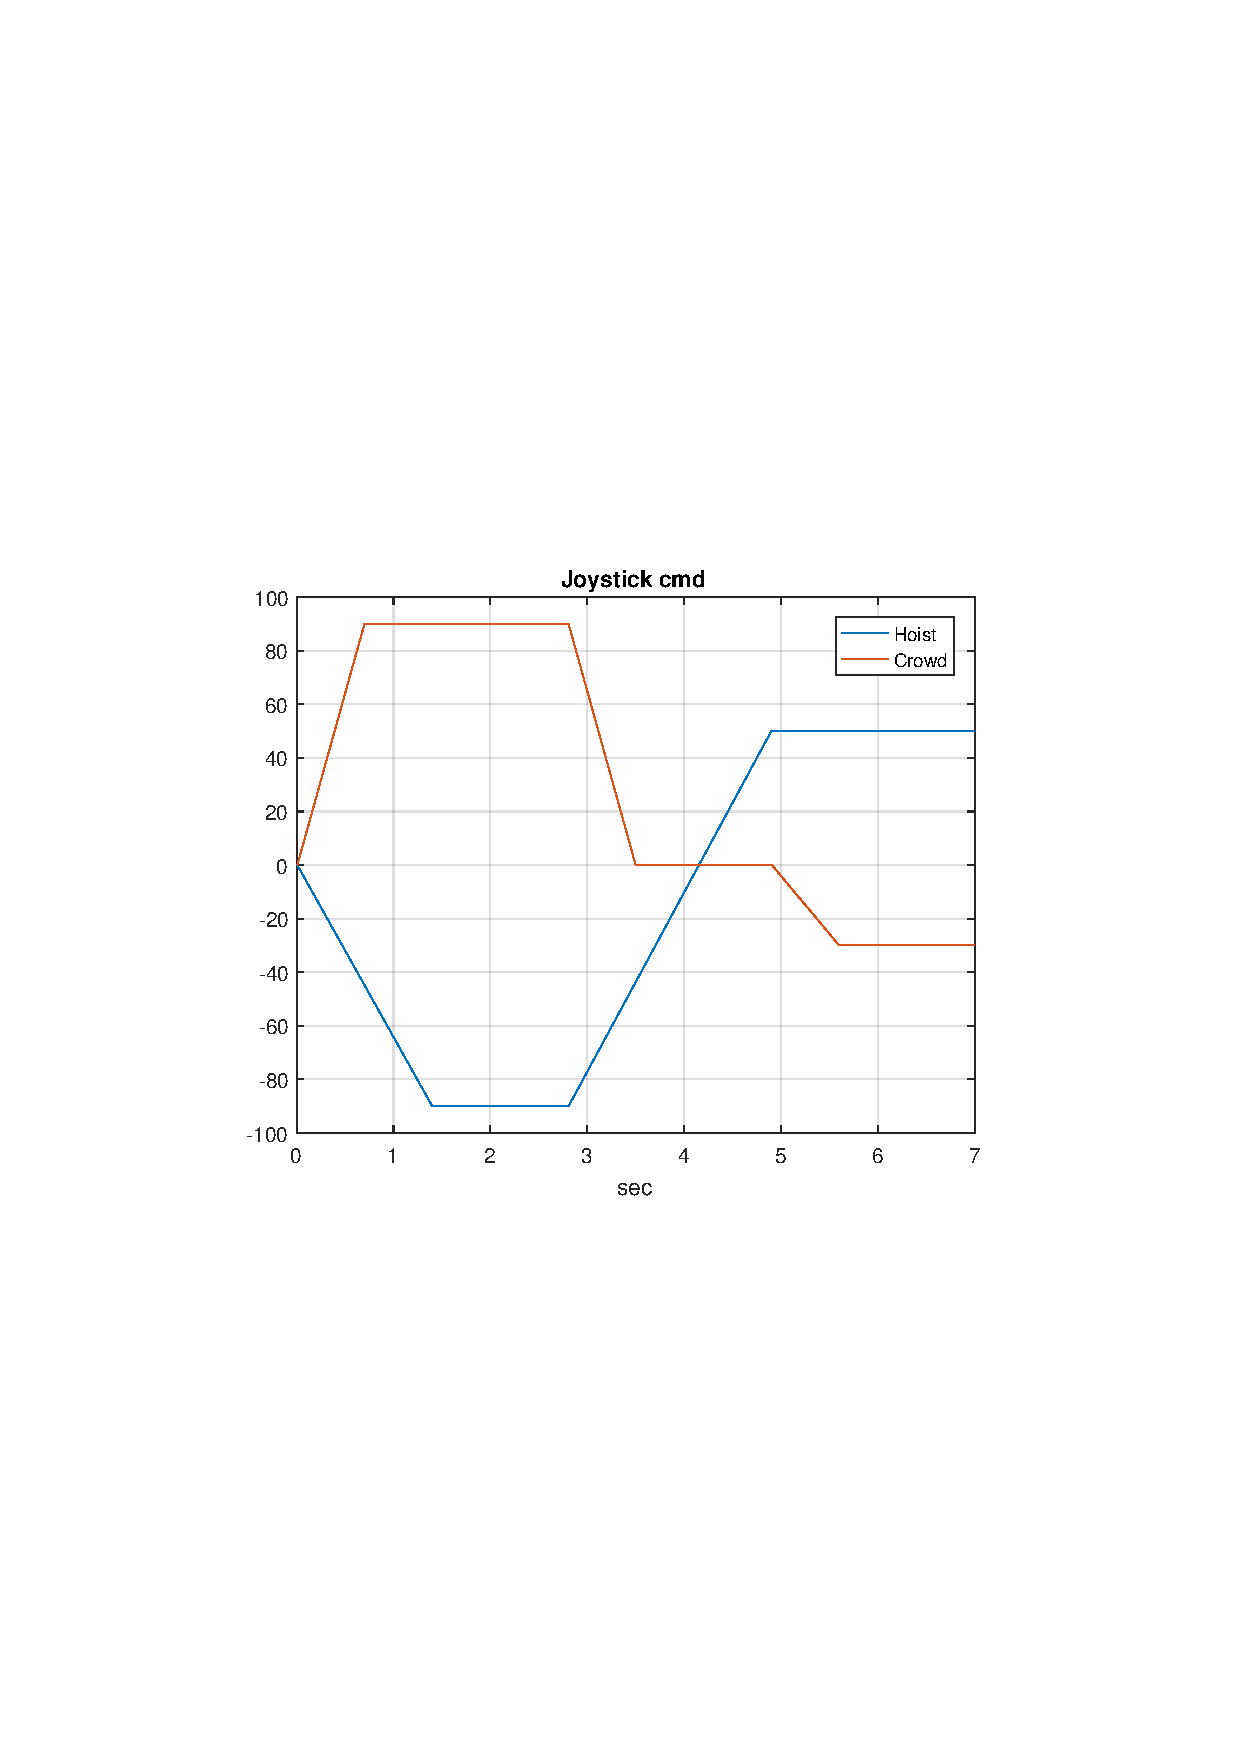
\includegraphics[trim=4cm 9cm 4cm 9.5cm, clip=true, width=\linewidth]{img/Joystick}
		\end{figure}
		\column{.5\textwidth}
		\onslide<3->
		\begin{figure}
			\centering
			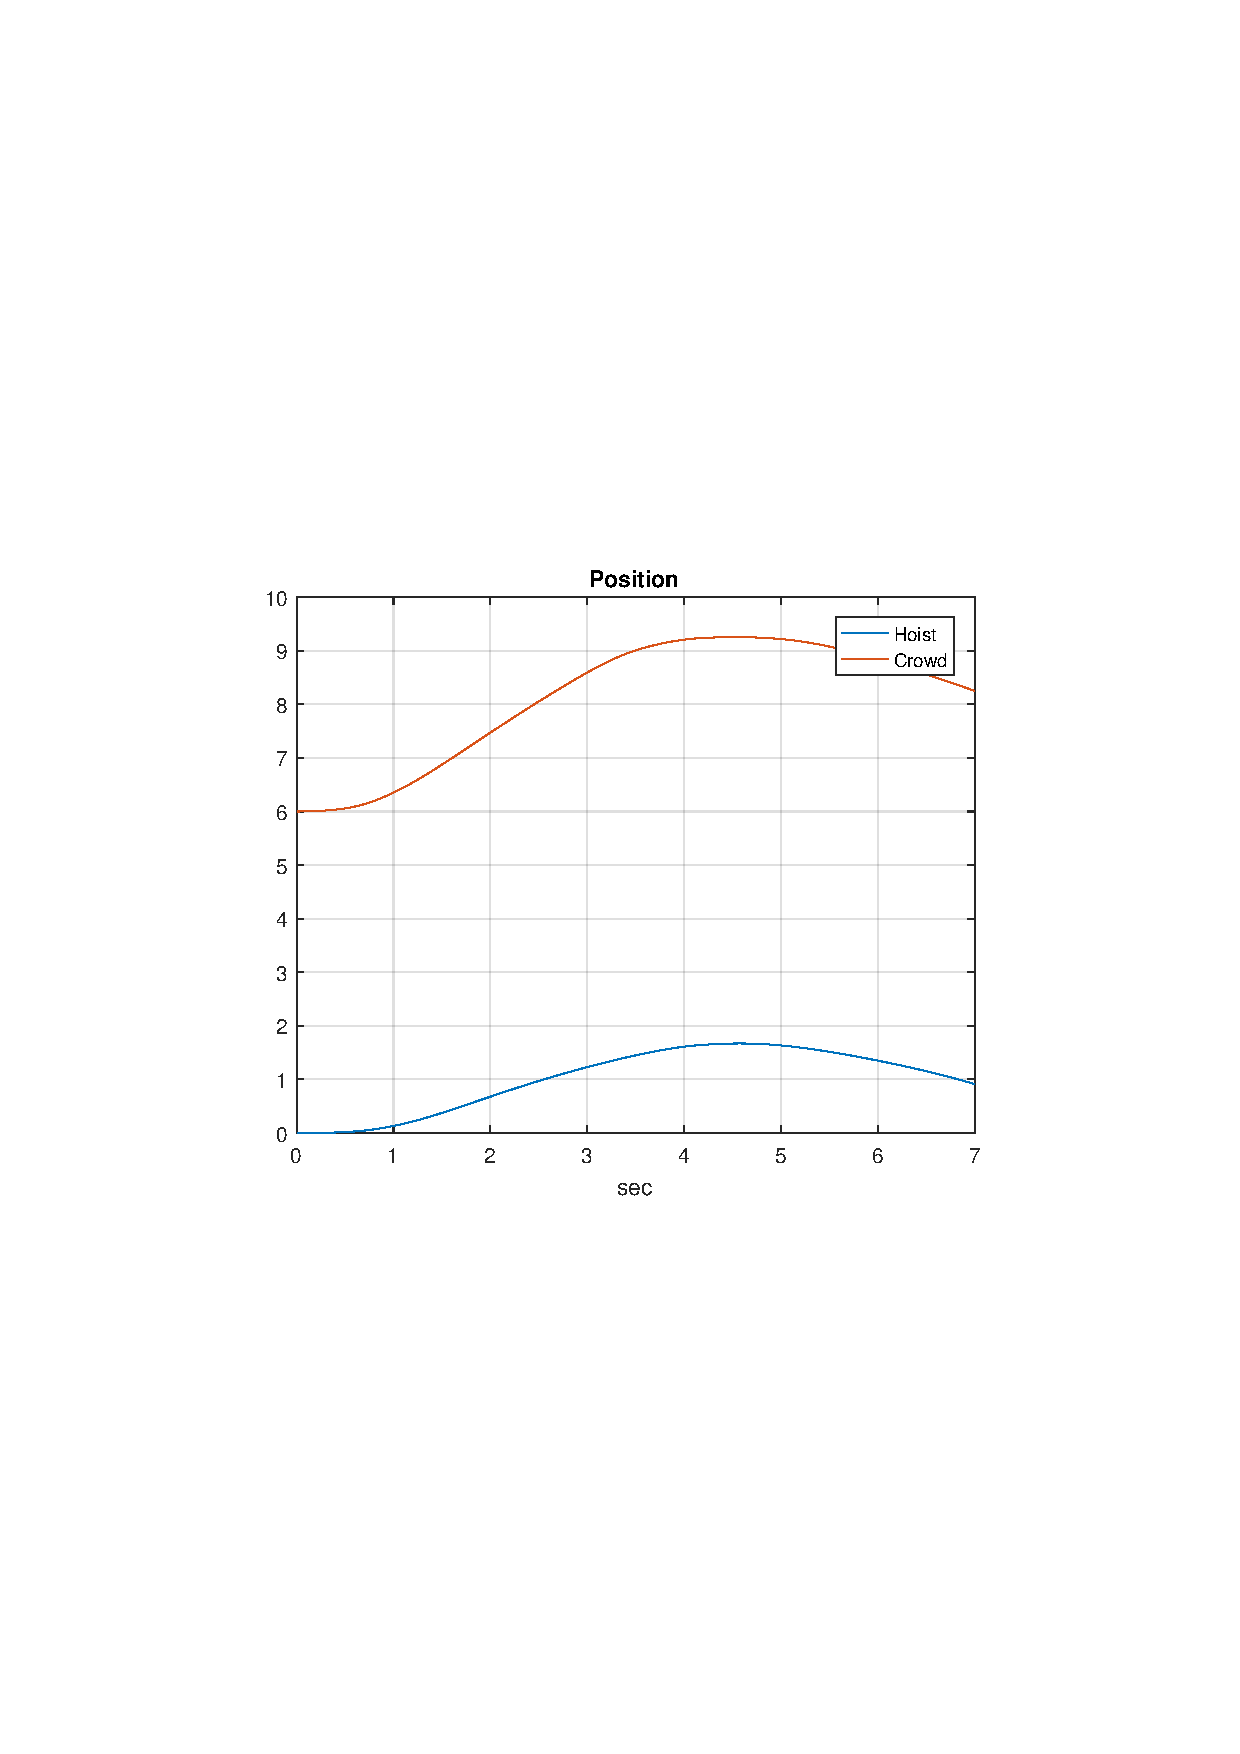
\includegraphics[trim=4cm 9cm 4cm 9.5cm, clip=true, width=\linewidth]{img/Position}
		\end{figure}
	\end{columns}
\end{frame}

\begin{frame}[c]
	\frametitle{Objective Function}
	\onslide<1->
		\textbf{Optimized Parameters:}
		\begin{itemize}
			\item{Inertia (Engine)}
			\item{Inertia (Arm)}
			\item{Friction}
			\item{Mass}
		\end{itemize}
	
		\vspace{.5cm}
	
	\onslide<2->
		\textbf{Penalty Term:}
		\vspace{-.5cm}
		\textcolor{white}{
		\begin{overprint}
			\onslide<2>
				\begin{align*}
					\min_{p\in\mathbb{R}^4}f(p) & = & & \frac 1 n \cdot \sum_{i=1}^{n}\left(\frac{\textcolor{black}{\Vert \overline{X}_i - X_i \left(p\right)\Vert^2}}{\Vert \overline{X}_i\Vert^2} + \frac{\Vert \overline{Y}_i - Y_i \left(p\right)\Vert^2}{\Vert \overline{Y}_i\Vert^2}\right) \\
					\operatorname{s.t.} & & & p_j \geq 0
				\end{align*}
			\onslide<3>
				\begin{align*}
					\min_{p\in\mathbb{R}^4}f(p) & = & & \frac 1 n \cdot \sum_{i=1}^{n}\left(\textcolor{black}{\frac{\Vert \overline{X}_i - X_i \left(p\right)\Vert^2}{\Vert \overline{X}_i\Vert^2}} + \frac{\Vert \overline{Y}_i - Y_i \left(p\right)\Vert^2}{\Vert \overline{Y}_i\Vert^2}\right) \\
					\operatorname{s.t.} & & & p_j \geq 0
				\end{align*}
			\onslide<4>
				\begin{align*}
					\min_{p\in\mathbb{R}^4}f(p) & = & & \frac 1 n \cdot \sum_{i=1}^{n}\left(\textcolor{black}{\frac{\Vert \overline{X}_i - X_i \left(p\right)\Vert^2}{\Vert \overline{X}_i\Vert^2} + \frac{\Vert \overline{Y}_i - Y_i \left(p\right)\Vert^2}{\Vert \overline{Y}_i\Vert^2}}\right) \\
					\operatorname{s.t.} & & & p_j \geq 0
				\end{align*}	
			\onslide<5>
				\begin{align*}
					\min_{p\in\mathbb{R}^4}f(p) & = & & \textcolor{black}{\frac 1 n \cdot \sum_{i=1}^{n}\left(\frac{\Vert \overline{X}_i - X_i \left(p\right)\Vert^2}{\Vert \overline{X}_i\Vert^2} + \frac{\Vert \overline{Y}_i - Y_i \left(p\right)\Vert^2}{\Vert \overline{Y}_i\Vert^2}\right)} \\
					\operatorname{s.t.} & & & p_j \geq 0
				\end{align*}
			\onslide<6->
				\textcolor{black}{
				\begin{align*}
					\min_{p\in\mathbb{R}^4}f(p) & = & & \frac 1 n \cdot \sum_{i=1}^{n}\left(\frac{\Vert \overline{X}_i - X_i \left(p\right)\Vert^2}{\Vert \overline{X}_i\Vert^2} + \frac{\Vert \overline{Y}_i - Y_i \left(p\right)\Vert^2}{\Vert \overline{Y}_i\Vert^2}\right) \\
					\operatorname{s.t.} & & & p_j \geq 0
				\end{align*}}
		\end{overprint}}
	
	\onslide<4->
		$\overline{X}_i$, $\overline{Y}_i$ reference trajectories
\end{frame}

\begin{frame}[c]
	\frametitle{Influence of the Parameters}
	\begin{columns}[c]
	
		\onslide<1->
		\column{.65\textwidth}
			10\% parameter deviation:
			\vspace{.5cm}
			\begin{itemize}
				\item{\makebox[3cm][l]{Inertia (Engine):} $1\cdot 10^{-3}$}
				\item{\makebox[3cm][l]{Inertia (Arm):} $3\cdot 10^{-3}$}
				\item{\makebox[3cm][l]{Friction:} $8\cdot 10^{-11}$}
				\item{\makebox[3cm][l]{Mass:} $5\cdot 10^{-2}$}
			\end{itemize}
			\vspace{.5cm}
		\onslide<2->
			Big parameter changes $\Rightarrow$ Small effects
		
		\onslide<3->
		\column{.35\textwidth}
			\vspace{-1.2cm}
			\begin{figure}
				\centering
				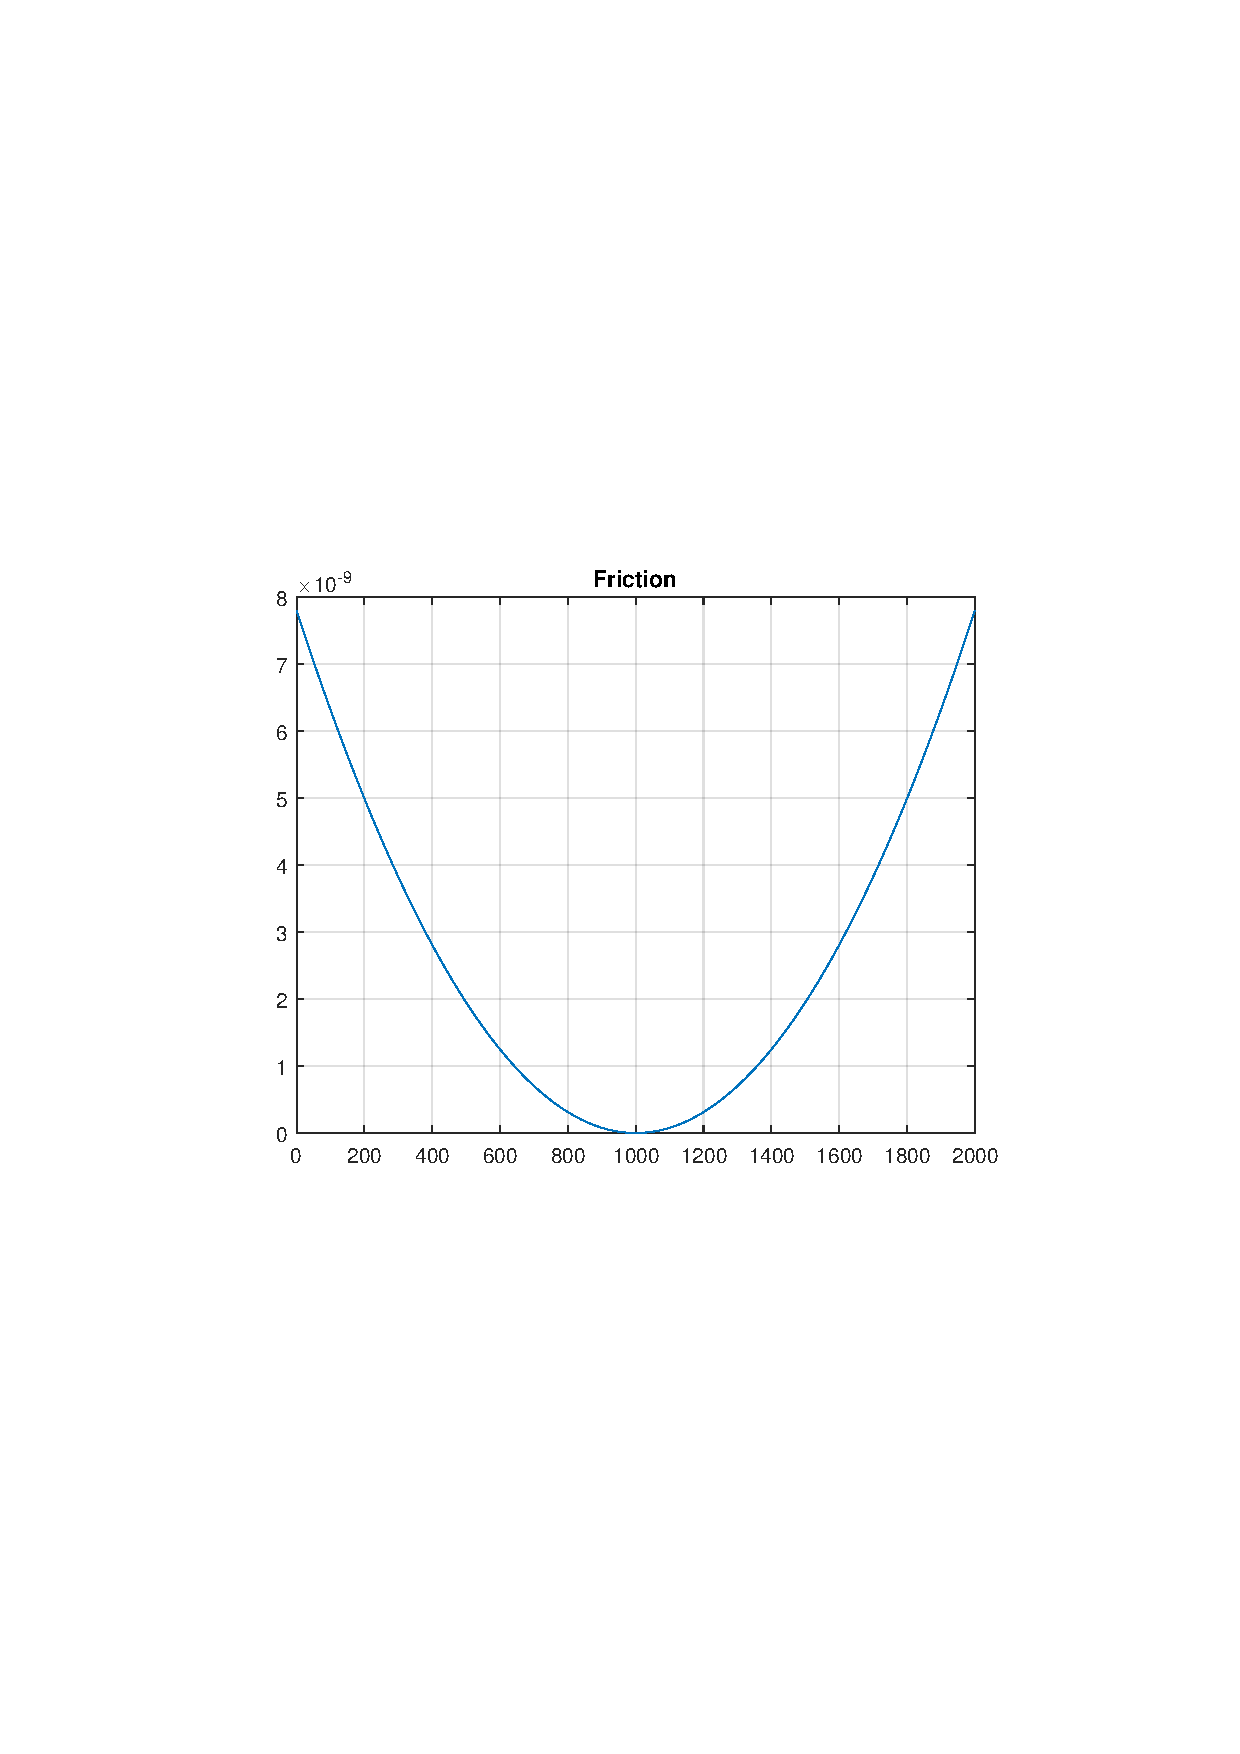
\includegraphics[trim=4cm 10cm 4cm 9.5cm, clip=true, width=\linewidth]{img/friction}
			\end{figure}
			\vspace{-0.6cm}
			\begin{figure}
				\centering
				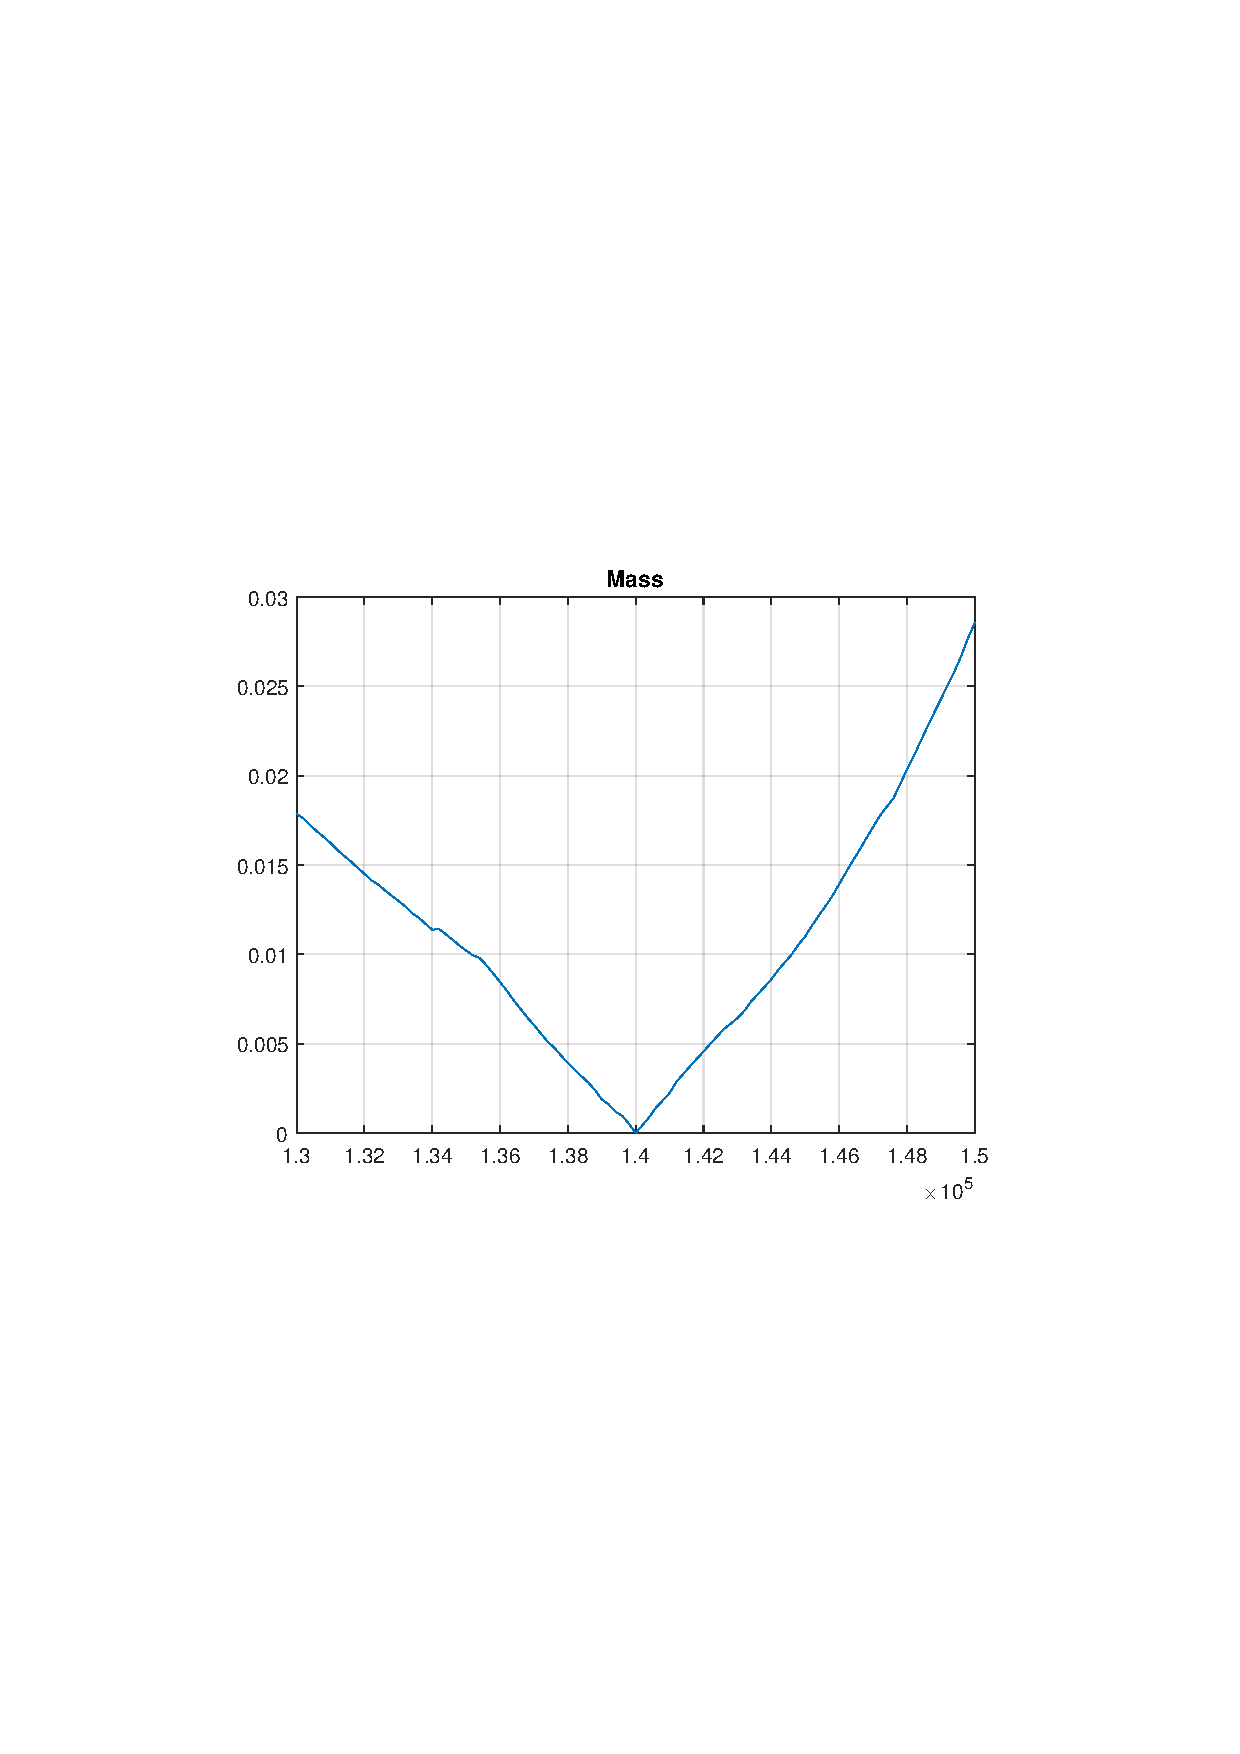
\includegraphics[trim=4cm 9cm 4cm 9.5cm, clip=true, width=\linewidth]{img/mass}
			\end{figure}
	\end{columns}
\end{frame}

\begin{frame}[c]
	\frametitle{Solvers}
	
	\onslide<1->
	\begin{itemize}
		\item{Derivative free optimization methods}
		\item{Deterministic or stochastic approaches}
		\item{Decrease function value by evaluating systematically}
	\end{itemize}
	\vspace{.5cm}
	
	\onslide<2->
	{\renewcommand{\arraystretch}{1.5}
	\begin{tabular}{l|lcrll}
		                    & value      & evaluations & time   & dev\raisebox{-.5ex}{\scriptsize{max}} & dev\raisebox{-.5ex}{\scriptsize{mean}} \\
		\hline
		Particle Swarm      & $10^{-12}$ & $2200$      & 6 min  & $10^{-1.0}$                           & $10^{-3.8}$                            \\
		Pattern Search      & $10^{-11}$ & $6500$      & 17 min & $10^{-1.3}$                           & $10^{-3.7}$                            \\
		Genetic Algorithm   & $10^{-4}$  & $5500$      & 14 min & $10^{-0.5}$                           & $10^{-1.0}$                            \\
		Simulated Annealing & $10^{-3}$  & $4200$      & 11 min & $10^{-0.3}$                           & $10^{-0.6}$                            \\
	\end{tabular}}
\end{frame}